% Options for packages loaded elsewhere
\PassOptionsToPackage{unicode}{hyperref}
\PassOptionsToPackage{hyphens}{url}
\PassOptionsToPackage{dvipsnames,svgnames,x11names}{xcolor}
%
\documentclass[
  a4paper,
]{scrreport}

\usepackage{amsmath,amssymb}
\usepackage{lmodern}
\usepackage{iftex}
\ifPDFTeX
  \usepackage[T1]{fontenc}
  \usepackage[utf8]{inputenc}
  \usepackage{textcomp} % provide euro and other symbols
\else % if luatex or xetex
  \usepackage{unicode-math}
  \defaultfontfeatures{Scale=MatchLowercase}
  \defaultfontfeatures[\rmfamily]{Ligatures=TeX,Scale=1}
\fi
% Use upquote if available, for straight quotes in verbatim environments
\IfFileExists{upquote.sty}{\usepackage{upquote}}{}
\IfFileExists{microtype.sty}{% use microtype if available
  \usepackage[]{microtype}
  \UseMicrotypeSet[protrusion]{basicmath} % disable protrusion for tt fonts
}{}
\makeatletter
\@ifundefined{KOMAClassName}{% if non-KOMA class
  \IfFileExists{parskip.sty}{%
    \usepackage{parskip}
  }{% else
    \setlength{\parindent}{0pt}
    \setlength{\parskip}{6pt plus 2pt minus 1pt}}
}{% if KOMA class
  \KOMAoptions{parskip=half}}
\makeatother
\usepackage{xcolor}
\setlength{\emergencystretch}{3em} % prevent overfull lines
\setcounter{secnumdepth}{5}
% Make \paragraph and \subparagraph free-standing
\ifx\paragraph\undefined\else
  \let\oldparagraph\paragraph
  \renewcommand{\paragraph}[1]{\oldparagraph{#1}\mbox{}}
\fi
\ifx\subparagraph\undefined\else
  \let\oldsubparagraph\subparagraph
  \renewcommand{\subparagraph}[1]{\oldsubparagraph{#1}\mbox{}}
\fi


\providecommand{\tightlist}{%
  \setlength{\itemsep}{0pt}\setlength{\parskip}{0pt}}\usepackage{longtable,booktabs,array}
\usepackage{calc} % for calculating minipage widths
% Correct order of tables after \paragraph or \subparagraph
\usepackage{etoolbox}
\makeatletter
\patchcmd\longtable{\par}{\if@noskipsec\mbox{}\fi\par}{}{}
\makeatother
% Allow footnotes in longtable head/foot
\IfFileExists{footnotehyper.sty}{\usepackage{footnotehyper}}{\usepackage{footnote}}
\makesavenoteenv{longtable}
\usepackage{graphicx}
\makeatletter
\def\maxwidth{\ifdim\Gin@nat@width>\linewidth\linewidth\else\Gin@nat@width\fi}
\def\maxheight{\ifdim\Gin@nat@height>\textheight\textheight\else\Gin@nat@height\fi}
\makeatother
% Scale images if necessary, so that they will not overflow the page
% margins by default, and it is still possible to overwrite the defaults
% using explicit options in \includegraphics[width, height, ...]{}
\setkeys{Gin}{width=\maxwidth,height=\maxheight,keepaspectratio}
% Set default figure placement to htbp
\makeatletter
\def\fps@figure{htbp}
\makeatother

%\newfontfamily\Ubuntu[Mapping=tex-text]{Ubuntu}
\usepackage{pgfplots}
\usetikzlibrary{arrows.meta,arrows}
\usetikzlibrary{angles,quotes}
\pgfplotsset{grid style={dashed,mygray}}
% Colors
\definecolor{myblue}{rgb}{0.067,0.529,0.871}
\definecolor{mypurple}{rgb}{0.859,0.071,0.525}
\definecolor{myred}{rgb}{1.0, 0.13, 0.32}
\definecolor{mygreen}{rgb}{0.01, 0.75, 0.24}
\definecolor{myblack}{gray}{0.1}
\definecolor{mygray}{gray}{0.8}
\newcommand{\NN}{\mathbb{N}}
\newcommand{\ZZ}{\mathbb{Z}}
\newcommand{\QQ}{\mathbb{Q}}
\newcommand{\RR}{\mathbb{R}}
\newcommand{\CC}{\mathbb{C}}
\DeclareMathOperator{\Int}{Int}
\DeclareMathOperator{\Ext}{Ext}
\DeclareMathOperator{\Fr}{Fr}
\DeclareMathOperator{\Adh}{Adh}
\DeclareMathOperator{\Ac}{Ac}
\DeclareMathOperator{\sen}{sen}
\makeatletter
\makeatother
\makeatletter
\@ifpackageloaded{bookmark}{}{\usepackage{bookmark}}
\makeatother
\makeatletter
\@ifpackageloaded{caption}{}{\usepackage{caption}}
\AtBeginDocument{%
\ifdefined\contentsname
  \renewcommand*\contentsname{Indice de contenidos}
\else
  \newcommand\contentsname{Indice de contenidos}
\fi
\ifdefined\listfigurename
  \renewcommand*\listfigurename{Listado de Figuras}
\else
  \newcommand\listfigurename{Listado de Figuras}
\fi
\ifdefined\listtablename
  \renewcommand*\listtablename{Listado de Tablas}
\else
  \newcommand\listtablename{Listado de Tablas}
\fi
\ifdefined\figurename
  \renewcommand*\figurename{Figura}
\else
  \newcommand\figurename{Figura}
\fi
\ifdefined\tablename
  \renewcommand*\tablename{Tabla}
\else
  \newcommand\tablename{Tabla}
\fi
}
\@ifpackageloaded{float}{}{\usepackage{float}}
\floatstyle{ruled}
\@ifundefined{c@chapter}{\newfloat{codelisting}{h}{lop}}{\newfloat{codelisting}{h}{lop}[chapter]}
\floatname{codelisting}{Listado}
\newcommand*\listoflistings{\listof{codelisting}{Listado de Listados}}
\makeatother
\makeatletter
\@ifpackageloaded{caption}{}{\usepackage{caption}}
\@ifpackageloaded{subcaption}{}{\usepackage{subcaption}}
\makeatother
\makeatletter
\@ifpackageloaded{tcolorbox}{}{\usepackage[many]{tcolorbox}}
\makeatother
\makeatletter
\@ifundefined{shadecolor}{\definecolor{shadecolor}{rgb}{.97, .97, .97}}
\makeatother
\makeatletter
\makeatother
\ifLuaTeX
\usepackage[bidi=basic]{babel}
\else
\usepackage[bidi=default]{babel}
\fi
\babelprovide[main,import]{spanish}
% get rid of language-specific shorthands (see #6817):
\let\LanguageShortHands\languageshorthands
\def\languageshorthands#1{}
\ifLuaTeX
  \usepackage{selnolig}  % disable illegal ligatures
\fi
\IfFileExists{bookmark.sty}{\usepackage{bookmark}}{\usepackage{hyperref}}
\IfFileExists{xurl.sty}{\usepackage{xurl}}{} % add URL line breaks if available
\urlstyle{same} % disable monospaced font for URLs
\hypersetup{
  pdftitle={Proyectos GIM},
  pdfauthor={Alfredo Sánchez Alberca},
  pdflang={es},
  colorlinks=true,
  linkcolor={blue},
  filecolor={Maroon},
  citecolor={Blue},
  urlcolor={Blue},
  pdfcreator={LaTeX via pandoc}}

\title{Proyectos GIM}
\usepackage{etoolbox}
\makeatletter
\providecommand{\subtitle}[1]{% add subtitle to \maketitle
  \apptocmd{\@title}{\par {\large #1 \par}}{}{}
}
\makeatother
\subtitle{Repositorio de casos prácticos}
\author{Alfredo Sánchez Alberca}
\date{6/1/22}

\begin{document}
\begin{titlepage}

%\AddToShipoutPicture*{\put(0,0){\includegraphics[scale=0.8]{img/background2}}} % Imagen de fondo, requiere el paquete eso-pic.
\begin{center}
\vspace*{5cm}

\Huge
{\textbf{\textsf{Proyectos GIM}}}

\vspace{0.5cm}
\LARGE
{\textbf{\textsf{Repositorio de casos prácticos}}}

\vspace{1.5cm}


\includegraphics[width=0.4\textwidth]{img/logos/proyectos.png}
\end{center}

\vfill

\begin{flushleft}
\begin{tabular}{ll}

\includegraphics[width=0.1\textwidth]{img/logos/aprendeconalf.png} & \parbox[b]{5cm}{\Large\textsf{Alfredo
Sánchez
Alberca}\\ \textsf{asalber@ceu.es} \\ \textsf{https://aprendeconalf.es}}
\end{tabular}
\end{flushleft}
\end{titlepage}\ifdefined\Shaded\renewenvironment{Shaded}{\begin{tcolorbox}[breakable, interior hidden, frame hidden, sharp corners, enhanced, boxrule=0pt, borderline west={3pt}{0pt}{shadecolor}]}{\end{tcolorbox}}\fi

\renewcommand*\contentsname{Indice de contenidos}
{
\hypersetup{linkcolor=}
\setcounter{tocdepth}{2}
\tableofcontents
}
\bookmarksetup{startatroot}

\hypertarget{prefacio}{%
\chapter*{Prefacio}\label{prefacio}}
\addcontentsline{toc}{chapter}{Prefacio}

\markboth{Prefacio}{Prefacio}

¡Bienvenida/os al repositorio de proyectos GIM!

Este repositorio contiene casos prácticos para desarrollar proyectos en
el grado de Ingeniería Matemática.

\hypertarget{licencia}{%
\section*{Licencia}\label{licencia}}
\addcontentsline{toc}{section}{Licencia}

\markright{Licencia}

Esta obra está bajo una licencia Reconocimiento -- No comercial --
Compartir bajo la misma licencia 3.0 España de Creative Commons. Para
ver una copia de esta licencia, visite
\url{https://creativecommons.org/licenses/by-nc-sa/3.0/es/}.

Con esta licencia eres libre de:

\begin{itemize}
\tightlist
\item
  Copiar, distribuir y mostrar este trabajo.
\item
  Realizar modificaciones de este trabajo.
\end{itemize}

Bajo las siguientes condiciones:

\begin{itemize}
\item
  \textbf{Reconocimiento} Debe reconocer los créditos de la obra de la
  manera especificada por el autor o el licenciador (pero no de una
  manera que sugiera que tiene su apoyo o apoyan el uso que hace de su
  obra).
\item
  \textbf{No comercial} No puede utilizar esta obra para fines
  comerciales.
\item
  \textbf{Compartir bajo la misma licencia} Si altera o transforma esta
  obra, o genera una obra derivada, sólo puede distribuir la obra
  generada bajo una licencia idéntica a ésta.
\end{itemize}

Al reutilizar o distribuir la obra, tiene que dejar bien claro los
términos de la licencia de esta obra.

Estas condiciones pueden no aplicarse si se obtiene el permiso del
titular de los derechos de autor.

Nada en esta licencia menoscaba o restringe los derechos morales del
autor.

\bookmarksetup{startatroot}

\hypertarget{demanda-eluxe9ctrica}{%
\chapter{Demanda eléctrica}\label{demanda-eluxe9ctrica}}

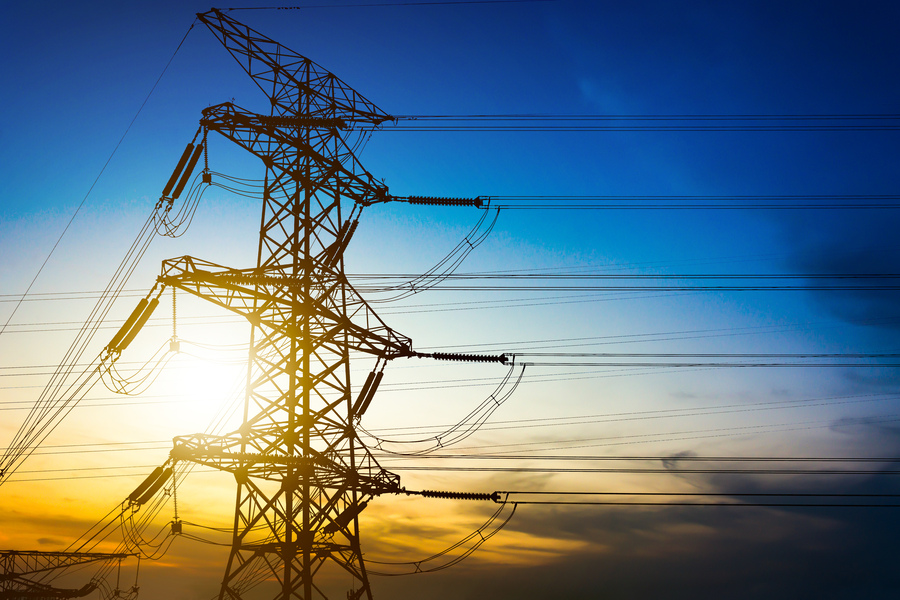
\includegraphics{./img/demanda-electrica/torre-electrica.jpg}

Las empresas energéticas necesitan predecir la demanda eléctrica de sus
clientes para poder dimensionar la producción y hacer una compra de
energía en el mercado diario. En este mercado se subasta la oferta de
energía para el día siguiente y las compañías comercializadoras pujan
para adquirir la potencia que estiman que sus clientes van a demandar en
las próximas 24 horas.

Para las compañías eléctricas comercializadoras es fundamental predecir
la curva de demanda de sus clientes, para ajustar la compra de energía a
las demandas reales, y para las compañías productoras es igualmente
importante predecir la demanda total para dimensionar la producción de
energía del día siguiente. Estas predicciones se realizan habitualmente
mediante complejos modelos matemáticos que combinan series temporales,
procesos estocásticos y aprendizaje automático.

\hypertarget{objetivos}{%
\section{Objetivos}\label{objetivos}}

En este proyecto no se pretende construir modelos predictivos, pero si
construir la curva de demanda eléctrica a partir de los consumos reales
en momentos puntuales. Es decir, se trata de desarrollar distintos
algoritmos de interpolación para ajustar la curva de demanda a una
muestra de consumos puntuales.

Para ello se utilizarán, al menos, los siguientes métodos:

\begin{itemize}
\tightlist
\item
  Interpolación polinómica:

  \begin{itemize}
  \tightlist
  \item
    Algebraica
  \item
    Método de Newton
  \item
    Método de Lagrange
  \end{itemize}
\item
  Interpolación mediante splines:

  \begin{itemize}
  \tightlist
  \item
    Splines lineales.
  \item
    Splines cuadráticos.
  \end{itemize}
\end{itemize}

\hypertarget{tareas}{%
\section{Tareas}\label{tareas}}

\begin{enumerate}
\def\labelenumi{\arabic{enumi}.}
\tightlist
\item
  Investigar los fundamentos matemáticos de los distintos métodos de
  interpolación.
\item
  Programar algoritmos para cada uno de los métodos de interpolación en
  Python o Julia.
\item
  Programar una interfaz para acceder a los datos de demanda eléctrica
  de mediante la API de Red Eléctrica.
\item
  Desarrollar una aplicación en la que el usuario final elija un día y
  un método de interpolación, y la aplicación le muestre las curva de
  demanda para ese día interpolada mediante el método seleccionado.
\end{enumerate}

\hypertarget{datos}{%
\section{Datos}\label{datos}}

Para probar los algoritmos de interpolación y la aplicación, se
utilizarán datos de la web \href{https://www.ree.es/}{Red Eléctrica}.
Esta web proporciona una \href{https://www.ree.es/es/apidatos}{API} que
permite acceder a base de datos de Red Eléctrica y que contiene, entre
otra mucha información, el histórico de demandas reales.

\bookmarksetup{startatroot}

\hypertarget{envuxedo-de-mensajes-en-una-red-de-telefonuxeda-muxf3vil}{%
\chapter{Envío de mensajes en una red de telefonía
móvil}\label{envuxedo-de-mensajes-en-una-red-de-telefonuxeda-muxf3vil}}

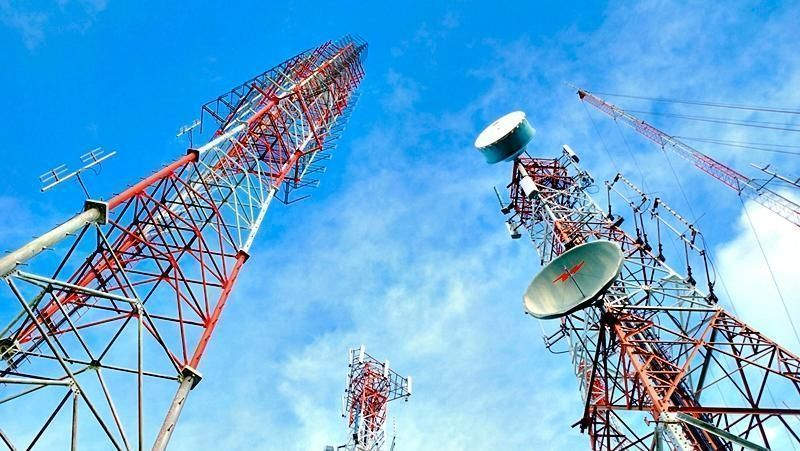
\includegraphics{./img/telefonia-movil/antenas.jpg}

La telefonía móvil utiliza una red de estaciones y subestaciones de
telecomunicación 4G para la transmisión de datos entre dispositivos
móviles. Muchas de estas estaciones están interconectadas por fibra y
otras se comunican mediante conexiones inalámbricas por radio
frecuencias.

Para que un mensaje llegue de un dispositivo emisor a otro receptor, el
mensaje debe recorrer el camino que va de la subestación más próxima al
emisor a la más próxima al receptor, pasando, a menudo, por varias
estaciones de la red que interconectan las subestaciones de origen y
destino. La distancia entre las estaciones y su capacidad de transmisión
de datos son claves para que los mensajes lleguen lo más rápidamente
posible del dispositivo emisor al receptor.

\hypertarget{objetivos-1}{%
\section{Objetivos}\label{objetivos-1}}

En este proyecto se debe desarrollar un algoritmo y una aplicación para
buscar el camino óptimo para enviar un mensaje desde un punto geográfico
a otro de una ciudad a través del grafo que representa la red de
estaciones y subestaciones de telecomunicación de la ciudad.

La aplicación recibirá como entrada las coordenadas de los puntos de
origen y destino, y el tamaño del mensaje, y debe devolver el camino más
rápido para enviar el mensaje del origen al destino, es decir, el orden
de las estaciones por las que el mensaje debe pasar, así como el tiempo
que el mensaje tardaría en recorrer ese camino. En la búsqueda del
camino óptimo debe tenerse en cuenta la distancia entre las
subestaciones, así como la capacidad de transmisión de cada una de
ellas.

Para la búsqueda del camino óptimo en el grafo conviene utilizar el
famoso
\href{https://es.wikipedia.org/wiki/Algoritmo_de_Dijkstra}{algoritmo de
Dijkstra} o alguna de sus variantes.

\hypertarget{tareas-1}{%
\section{Tareas}\label{tareas-1}}

\begin{enumerate}
\def\labelenumi{\arabic{enumi}.}
\tightlist
\item
  Obtener las coordenadas geográficas de la ubicación de las estaciones
  de telefonía con una frecuencia específica y de un único operador en
  una determinada ciudad y representar la red en un plano cartesiano. Se
  puede asumir que las estaciones a menos de \(x\) kilómetros de
  separación están directamente conectadas por fibra.
\item
  Construir un grafo que represente la red de estaciones de telefonía.
  Los pesos de las aristas del grafo podrían ser las distancias en línea
  recta entre las estaciones, pero es mucho más realista es utilizar la
  velocidad de conexión entre ellas en Mbps, ya que las estaciones base
  suelen conectarse entre ellas con conexiones inalámbricas. Para ello
  se puede utilizar la capacidad de Shannon como se explica en este
  \href{https://dspace.networks.imdea.org/bitstream/handle/20.500.12761/689/main_Throughput_MiSARN2019_CameraReady_Embedded_CertifiedIEEEeXplore.pdf?sequence=1}{artículo}.
\item
  Identificar en el grafo las estaciones base más cercanas a las
  coordenadas de los puntos de origen y destino del mensaje.
\item
  Implementar en Python o Julia el algoritmo de Dijkstra o alguna de sus
  variantes para la búsqueda del camino óptimo.
\item
  Determinar cuál será la estación base que requiera más atención de
  mantenimiento, es decir, por la que pasen más mensajes. Para ello,
  usar la métrica de centralidad correspondiente. O lo que es lo mismo,
  si hubiera un agente malicioso (a.k.a. man in the middle, o Charlie),
  ¿dónde se ubicaría para interceptar la mayoría de mensajes.
\item
  Determinar cuánto tardará como máximo un mensaje en llegar de emisor a
  receptor. Usar la matriz de distancias tras ejecutar el algoritmo de
  Dijkstra y calcular el diámetro del grafo.
\end{enumerate}

\hypertarget{datos-1}{%
\section{Datos}\label{datos-1}}

Para probar obtener los datos de la ubicación y frecuencia de
transmisión de las estaciones de telefonía de una determinada ciudad
puede consultarse
\href{https://geoportal.minetur.gob.es/VCTEL/vcne.do}{web del Ministerio
de Asuntos Económicos y Transformación Digital} o bien esta otra web con
el \href{https://antenasgsm.com/}{mapa de estaciones de telefonía del
Estado español}.

\bookmarksetup{startatroot}

\hypertarget{convive-big-data-para-la-ciudad-inteligente}{%
\chapter{CONVIVE: Big Data para la ciudad
inteligente}\label{convive-big-data-para-la-ciudad-inteligente}}

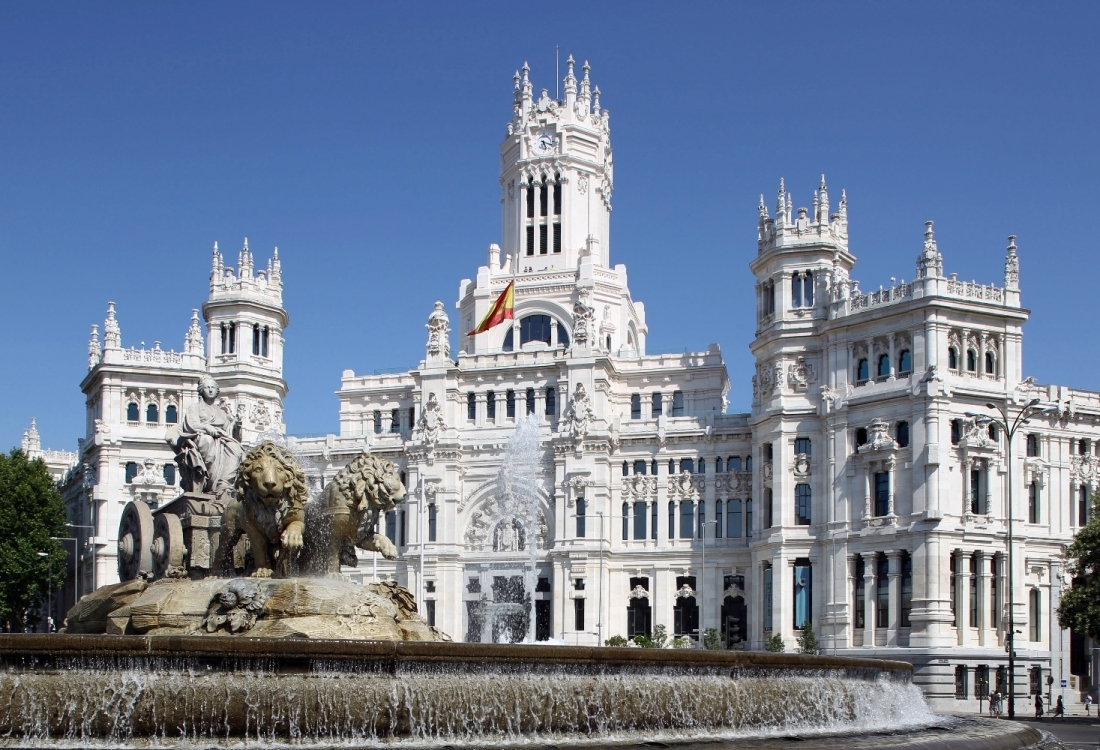
\includegraphics{./img/convive/ayuntamiento-madrid.jpg}

Los datos abiertos (open data) es una iniciativa que muchas
administraciones públicas están adoptando con el objetivo de mejorar la
transparencia en lo que respecta a sus funciones de cara a la
ciudadanía.

El ayuntamiento de Madrid es uno de los ayuntamientos que ha empezado a
ofrecer datos en abierto, y en su portal de datos abiertos puede
accederse a multitud de bases de datos con información de todo tipo,
desde los alojamientos en la ciudad hasta las mediciones de
contaminación de las estaciones de registro de contaminantes.

La puesta a disposición de la ciudadanía de toda esta información, no
solo mejora la transparencia sobre la gestión municipal, sino que
permite a ciudadanos o a empresas particulares poder analizar estos
datos para mejorar sus decisiones.

\hypertarget{objetivos-2}{%
\section{Objetivos}\label{objetivos-2}}

El objetivo principal del proyecto CONVIVE es mejorar el conocimiento
del estado real de la ciudad a través de la medición de datos de su
entorno y de la información aportada por los ciudadanos. Para ello se
desplegará toda la infraestructura necesaria para adquirir esa
información y tratarla adecuadamente.

Un objetivo específico del proyecto es que el tratamiento de datos debe
realizarse con tecnologías relacionadas con el Big Data. Así nos
aseguraremos de que el sistema pueda integrar fuentes de información
variadas incluso después de que el sistema haya sido creado.

\hypertarget{descripciuxf3n-tuxe9cnica}{%
\section{Descripción técnica}\label{descripciuxf3n-tuxe9cnica}}

El sistema a implementar consiste en una plataforma de análisis de
varias fuentes de información existentes en el Ayuntamiento de Madrid.
Para ello debe solucionar tres aspectos fundamentales:

\begin{enumerate}
\def\labelenumi{\arabic{enumi}.}
\tightlist
\item
  La recogida de información de la ciudad. Este sistema incluye datos de
  dispositivos, de ciudadanos y de entidades.
\item
  La gestión de los datos recogidos. Debe ser lo suficientemente
  genérica para gestionar posibles incertidumbres en los datos propias
  de una ciudad: información incompleta, nuevas fuentes de información,
  nuevos campos en la misma información, etc.
\item
  El análisis de los datos almacenados. Los análisis pueden basarse en
  la combinación de varios conjuntos de datos integrados en el sistema.
  Es necesario tener en cuenta que estos datos pueden estar en
  ubicaciones diferentes y pueden tener un tamaño que no permita su
  adecuado procesamiento en una sola máquina.
\end{enumerate}

En una ciudad el número de fuentes de información no está fijado ya que
en cualquier momento pueden aparecer nuevas fuentes de información a
medida que se implanten tecnologías nuevas o formas distintas de
participar por parte de los ciudadanos. En el proyecto CONVIVE se
definen algunas fuentes de información que deben ser tratadas y se
emplean tecnologías que faciliten la integración de nuevas fuentes de
información en el futuro. Las fuentes de información que debe gestionar
CONVIVE son:

\begin{itemize}
\tightlist
\item
  Avisos de incidencias en la vía pública por parte de los ciudadanos.
  El sistema integrará estos avisos tanto de forma interactiva (para
  gestionar la incidencia) como de forma procesada (registros de avisos
  durante un periodo de tiempo).

  \begin{itemize}
  \tightlist
  \item
    Los avisos interactivos se almacenarán en un sistema que permita la
    actualización del estado de los mismos.
  \item
    Los avisos procesados suelen corresponder a avisos interactivos que
    han sido transformados a un formato que facilita su procesamiento
    estadístico. De esta forma se podrá relacionar estos avisos con
    otras fuentes estadísticas disponibles en la ciudad.
  \end{itemize}
\item
  Información acústica de la ciudad. El sistema integrará los datos del
  nivel de ruido existente en distintas partes de la ciudad. Para ello
  obtendrá la información de ruido en determinadas zonas y los
  registrará para su posterior análisis.
\end{itemize}

Para llevar a cabo el proyecto CONVIVE se divide su desarrollo en tres
subsistemas distintos que coinciden con los tres aspectos a solucionar
previamente comentados.

\hypertarget{subsistema-de-adquisiciuxf3n-de-datos}{%
\subsection{Subsistema de adquisición de
datos}\label{subsistema-de-adquisiciuxf3n-de-datos}}

En este subsistema de deben solucionar aspectos relacionados con la
recogida de la información. Para ello debe desplegar una red de sensores
acústicos en la ciudad (encargados del proceso de recogida de
información de ruido) y habilitar un sistema de comunicación para los
ciudadanos (con el fin de generar avisos de incidencias en la vía
pública).

En el proyecto CONVIVE tendremos dos tipos de información al finalizar
el trabajo en este subsistema:

\begin{enumerate}
\def\labelenumi{\arabic{enumi}.}
\tightlist
\item
  Una base de datos con información sobre las incidencias reportadas por
  los ciudadanos. En esta base de datos se almacenan las incidencias
  activas y cuyo estado se puede actualizar. Como criterio de diseño se
  almacenarán en una base de datos (no en un fichero) ya que tiene
  ciertas ventajas para su gestión.
\item
  Información relacionada con los niveles de ruido. Se recogerá
  información de los sensores desplegados en la ciudad y se almacenarán
  en ficheros con formato CSV.
\end{enumerate}

\begin{figure}

{\centering 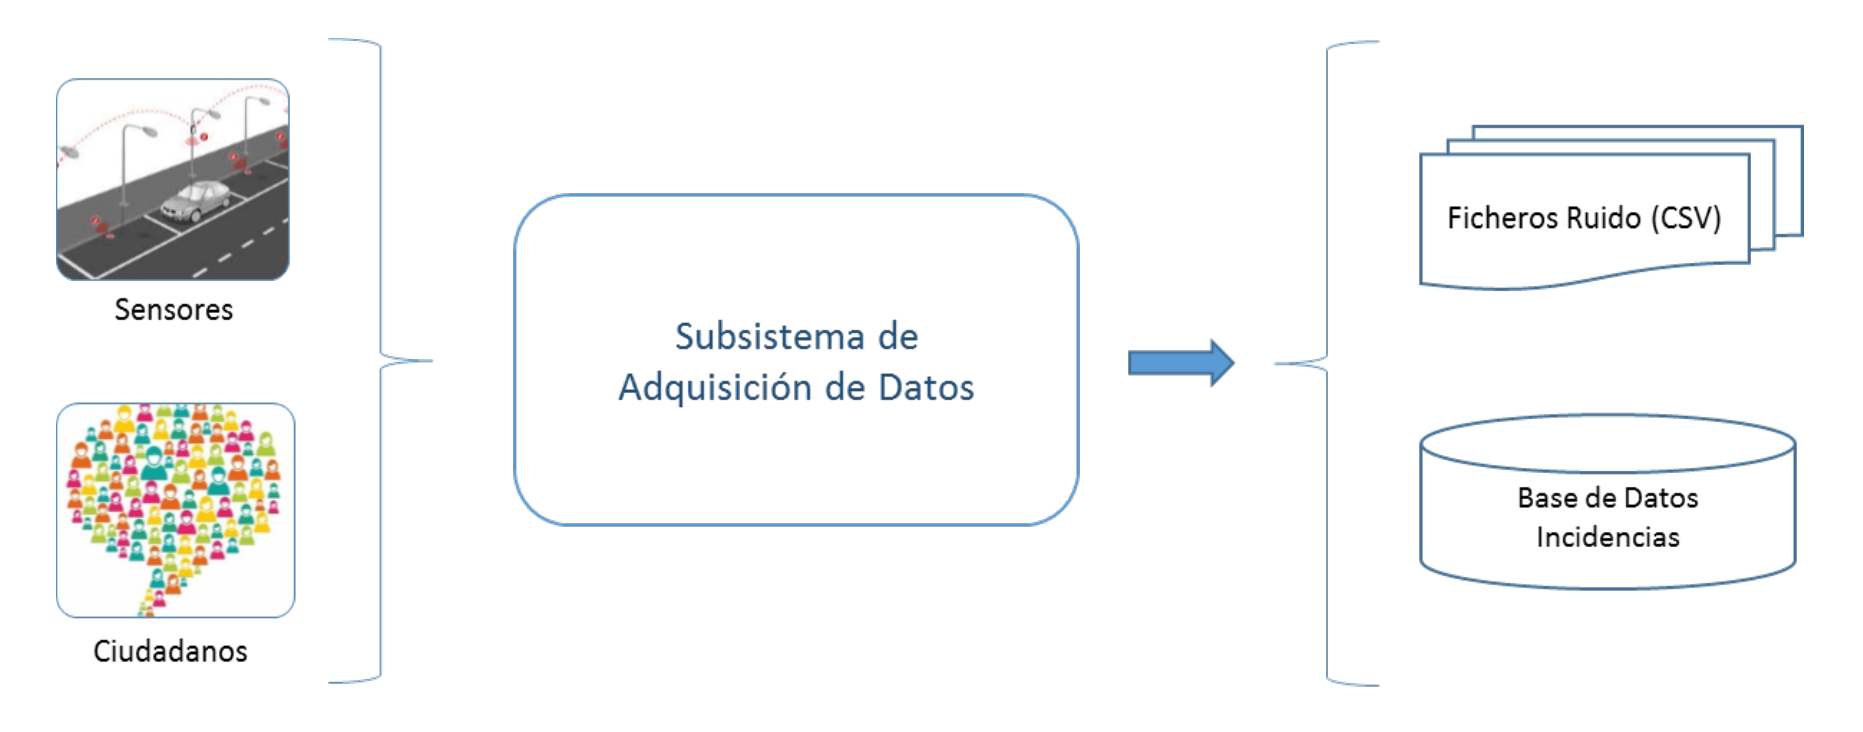
\includegraphics{./img/convive/subsistema-adquisicion-datos.png}

}

\caption{Subsistema de adquisición de datos}

\end{figure}

\hypertarget{subsistema-de-gestiuxf3n-de-datos}{%
\subsection{Subsistema de gestión de
datos}\label{subsistema-de-gestiuxf3n-de-datos}}

En este subsistema de deben solucionar aspectos relacionados con el
almacenamiento y sincronización de la información a través de distintas
máquinas.

Dado que no se implementará realmente el subsistema de adquisición de
datos (aunque sí se llevará a cabo un diseño detallado), se obtendrán
datos del sistema AVISA que contiene las incidencias reportadas por los
ciudadanos, y del nivel de ruidos del Ayuntamiento de Madrid.

Una vez que se disponga de todos los datos como ficheros en formato CSV
(los datos de AVISA y los de ruido) utilizaremos un sistema que permita
distribuirlos a través de varias máquinas y sincronizarlos para
facilitar su acceso.

\begin{figure}

{\centering 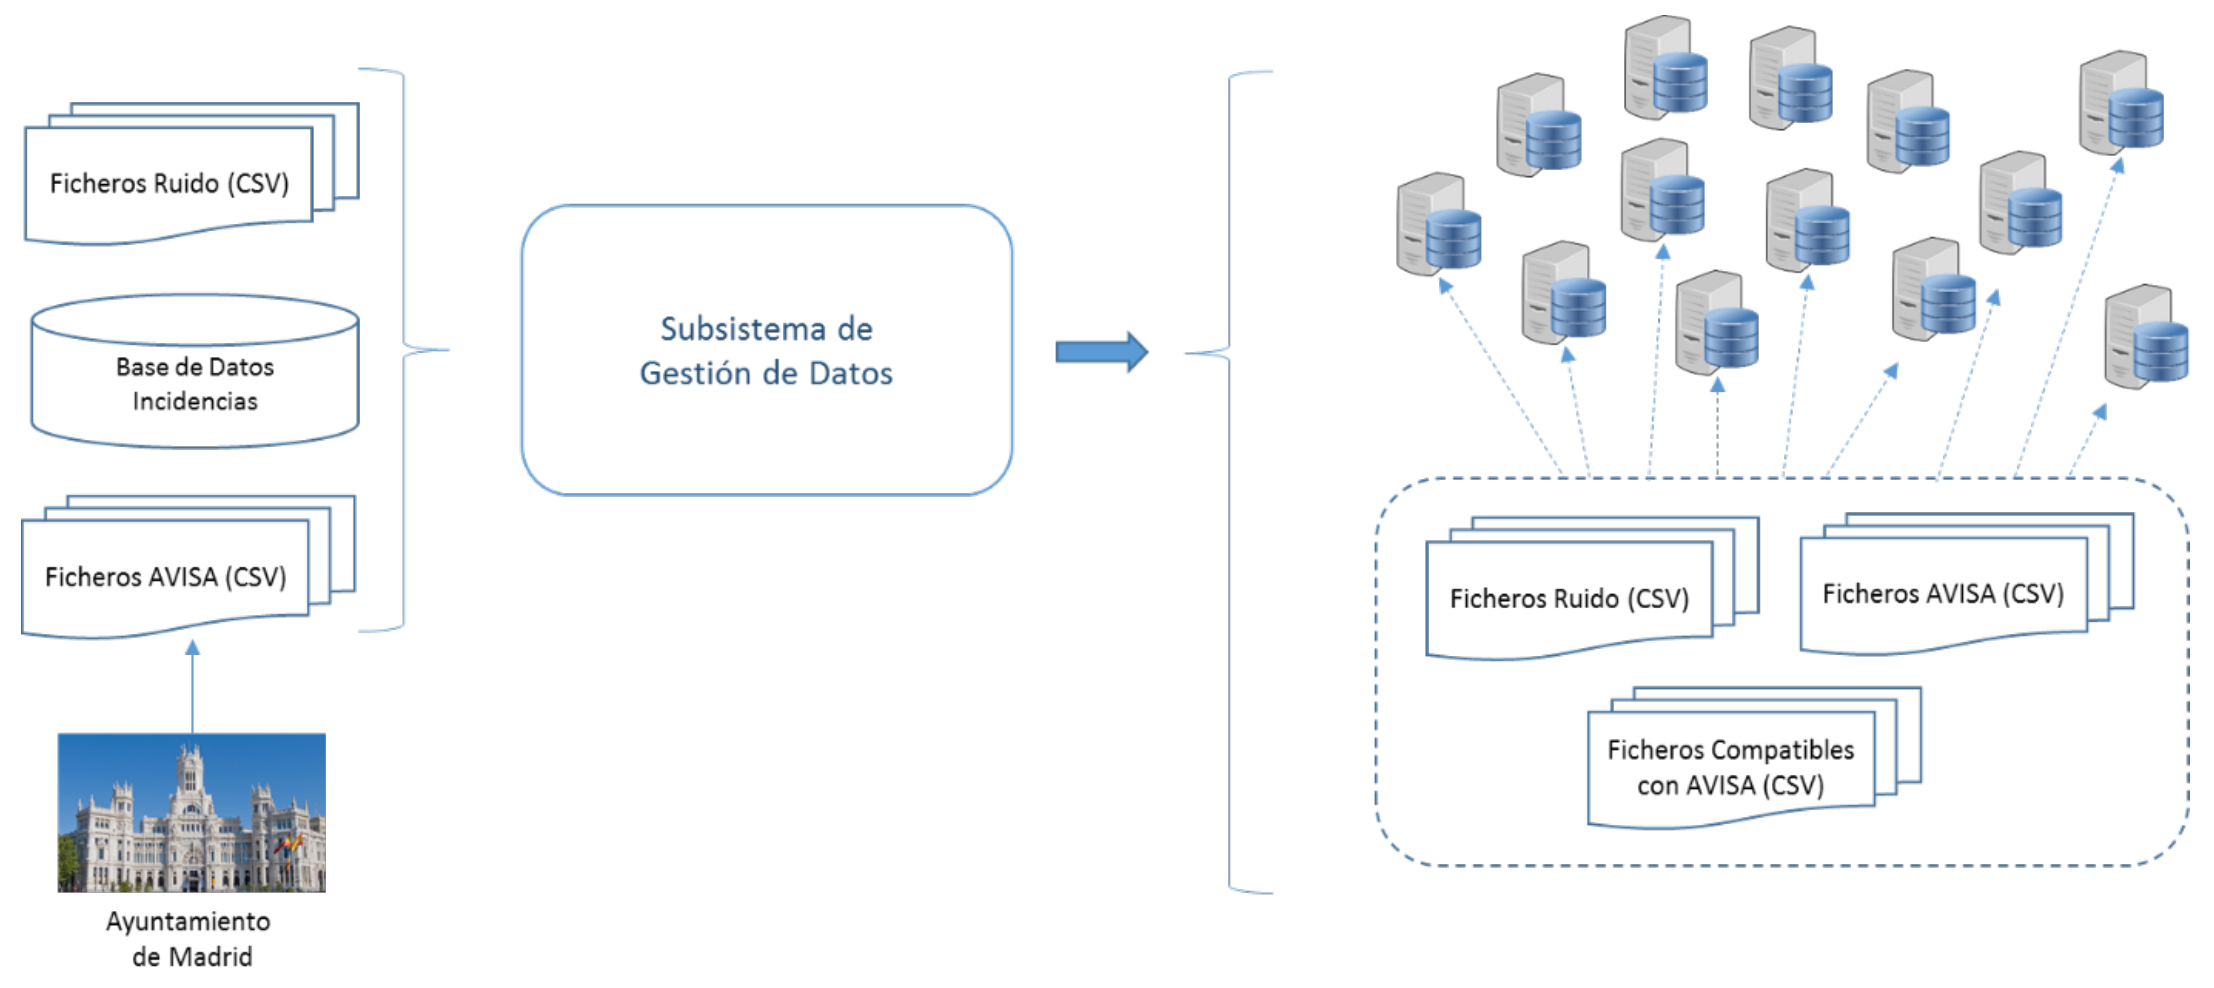
\includegraphics{./img/convive/subsistema-gestion-datos.png}

}

\caption{Subsistema de gestión de datos}

\end{figure}

\hypertarget{subsistema-de-anuxe1lisis-de-datos}{%
\subsection{Subsistema de análisis de
datos}\label{subsistema-de-anuxe1lisis-de-datos}}

En este subsistema se obtiene información útil a partir de todos los
datos disponibles. En un sistema real se cruzarían los datos del sistema
AVISA, con los de niveles de ruido y con varios datos más para obtener
información sintetizada y en muchos casos inferir relaciones entre
distintos hechos que estén ocurriendo. En el caso del proyecto CONVIVE,
por motivos de claridad a la hora de aprender conceptos, se utilizará
únicamente un fichero con los datos del sistema AVISA en formato CSV. Se
descartarán tanto los datos de ruido como cualquier otro tipo de fuente
de datos que puede obtenerse del Ayuntamiento de Madrid.

En el proyecto CONVIVE se realizarán dos acciones con los datos:

\begin{enumerate}
\def\labelenumi{\arabic{enumi}.}
\item
  Se analizarán los datos existentes del sistema AVISA para obtener
  información sintetizada de los incidentes reportados. Para ello debe
  tenerse en cuenta que el fichero con los datos puede estar repartido
  entre varias máquinas y que se debe utilizar un modelo de programación
  que facilite el acceso a todos esos datos sin cargar la máquina en la
  que se ejecute.
\item
  Se visualizarán los datos del sistema AVISA para que sean más
  fácilmente entendibles por los destinatarios finales. Las decisiones
  finales sobre las acciones a tomar las llevarán a cabo por personas
  con distintas capacidades de abstracción y síntesis. Para facilitar
  esas decisiones se mostrarán los datos mediante modelos visuales que
  permitan una mejor comprensión de éstos.
\end{enumerate}

\begin{figure}

{\centering 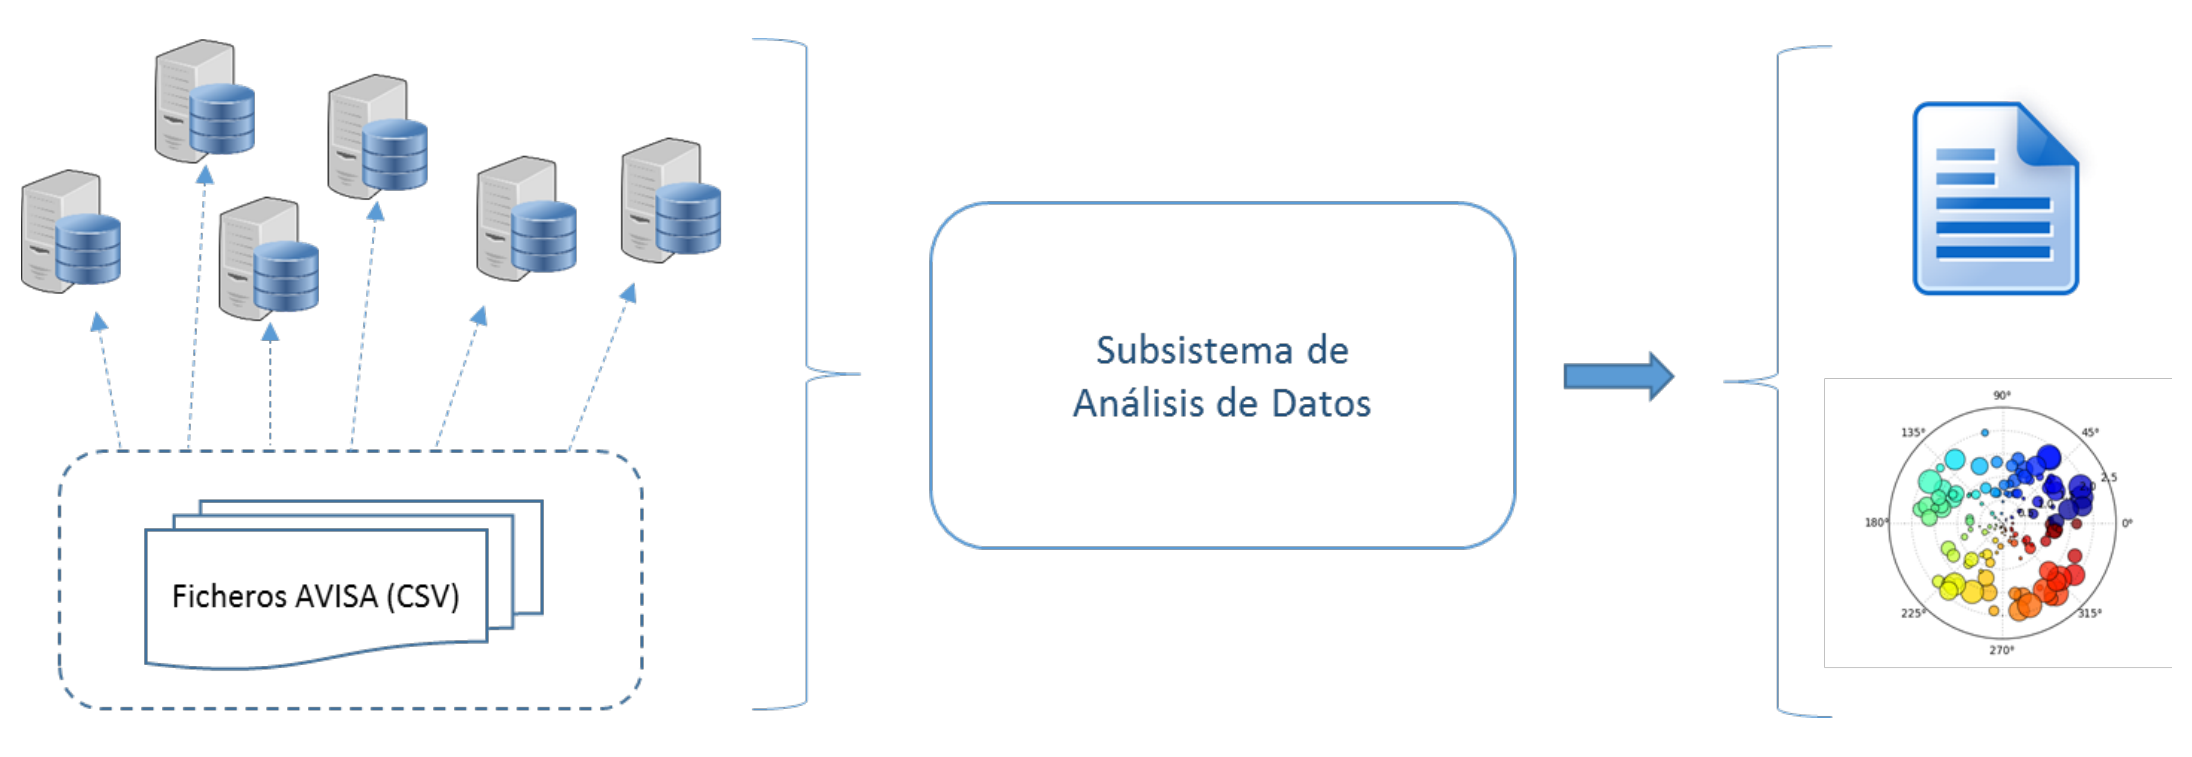
\includegraphics{./img/convive/subsistema-analisis-datos.png}

}

\caption{Subsistema de análisis de datos}

\end{figure}

\hypertarget{tareas-2}{%
\section{Tareas}\label{tareas-2}}

\begin{enumerate}
\def\labelenumi{\arabic{enumi}.}
\tightlist
\item
  Obtener los ficheros de datos del sistema AVISA del Ayuntamiento de
  Madrid.
\item
  Obtener los ficheros de ruido del Ayuntamiento de Madrid.
\item
  Crear el procedimiento de transformación de entradas de la base de
  datos en ficheros en formato compatible con los del sistema AVISA.
\item
  Incluir todos los ficheros, los del sistema AVISA, los generados a
  partir de la base de datos y los de ruido, en un sistema de ficheros
  distribuido.
\item
  Preprocesar el conjunto de datos para prepararlo para el análisis
  estadístico.
\item
  Realizar un análisis estadístico de las principales variables
  incluidas en el conjunto de datos.
\item
  Crear gráficos de visualización de los datos correspondientes a las
  principales variables del conjunto de datos.
\end{enumerate}

\hypertarget{datos-2}{%
\section{Datos}\label{datos-2}}

Se obtendrán ficheros con información del
\href{http://datos.madrid.es/portal/site/egob}{portal de datos abiertos
del Ayuntamiento de Madrid}. Este portal tiene un catálogo de datos
disponibles bajo los principios de la iniciativa Datos Abiertos (Open
Data), que impulsa la publicación abierta, regular, reutilizable y
autorizada de los datos de carácter público. En concreto se utilizarán
los conjuntos de datos siguientes:

\begin{itemize}
\tightlist
\item
  Datos del Sistema AVISA. Tiene información de avisos de ciudadanos
  sobre incidencias en la vía pública. Es un fichero en formato CSV.
\item
  Información de la contaminación acústica. Es otro fichero en formato
  CSV.
\end{itemize}

\bookmarksetup{startatroot}

\hypertarget{sistema-de-cuxe1lculo-simbuxf3lico-de-derivadas}{%
\chapter{Sistema de cálculo simbólico de
derivadas}\label{sistema-de-cuxe1lculo-simbuxf3lico-de-derivadas}}

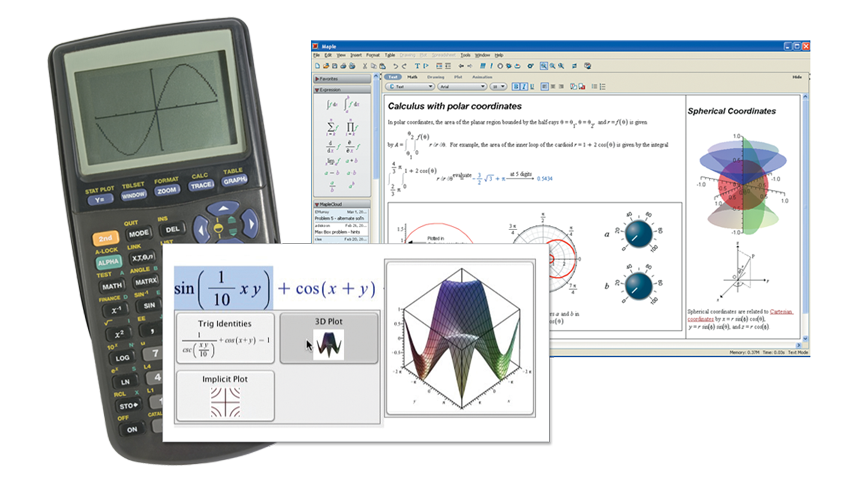
\includegraphics{./img/calculo-simbolico-derivadas/cas.png}

Un \emph{sistema de álgebra computacional} (CAS, del inglés computer
algebra system) es un programa de ordenador o calculadora avanzada que
facilita el cálculo simbólico. La principal diferencia entre un CAS y
una calculadora tradicional es la habilidad del primero para trabajar
con ecuaciones y fórmulas simbólicamente, en lugar de numéricamente.
Esto permite trabajar con expresiones simbólicas (no numéricas) y
realizar operaciones como la resolución de ecuaciones, el cálculo de
límites, el cálculo de derivadas o el cálculo de integrales.

\hypertarget{objetivos-3}{%
\section{Objetivos}\label{objetivos-3}}

El objetivo de este proyecto es desarrollar un sistema de álgebra
computacional para el cálculo simbólico de derivadas.

\hypertarget{tareas-3}{%
\section{Tareas}\label{tareas-3}}

\begin{enumerate}
\def\labelenumi{\arabic{enumi}.}
\tightlist
\item
  Definir simbólicamente las derivadas de las funciones elementales.
\end{enumerate}



\end{document}
